\documentclass[12pt, a4paper]{report}
\usepackage[utf8]{inputenc}
\usepackage[english, russian]{babel}

\usepackage{graphicx}
\usepackage{listings}
\usepackage{color}

\usepackage{amsmath}
\usepackage{pgfplots}
\usepackage{url}
\usepackage{flowchart}
\usepackage{tikz}
\DeclareGraphicsExtensions{.pdf,.png,.jpg,.svg}
\usetikzlibrary{shapes, arrows}

\usepackage{pgfplotstable}

\renewcommand\contentsname{Содержание}

\usepackage{geometry}
\geometry{left=3cm}
\geometry{right=1cm}
\geometry{top=2cm}
\geometry{bottom=2cm}

\lstset{ %
language=C++,                 % выбор языка для подсветки (здесь это С)
basicstyle=\small\sffamily, % размер и начертание шрифта для подсветки кода
numbers=left,               % где поставить нумерацию строк (слева\справа)
numberstyle=\tiny,           % размер шрифта для номеров строк
stepnumber=1,                   % размер шага между двумя номерами строк
numbersep=-5pt,                % как далеко отстоят номера строк от         подсвечиваемого кода
backgroundcolor=\color{white}, % цвет фона подсветки - используем         \usepackage{color}
showspaces=false,            % показывать или нет пробелы специальными     отступами
showstringspaces=false,      % показывать или нет пробелы в строках
showtabs=false,             % показывать или нет табуляцию в строках
frame=single,              % рисовать рамку вокруг кода
tabsize=2,                 % размер табуляции по умолчанию равен 2 пробелам
captionpos=t,              % позиция заголовка вверху [t] или внизу [b] 
breaklines=true,           % автоматически переносить строки (да\нет)
breakatwhitespace=false, % переносить строки только если есть пробел
escapeinside={\%*}{*)},   % если нужно добавить комментарии в коде
keywordstyle=\color{blue}\ttfamily,
stringstyle=\color{red}\ttfamily,
commentstyle=\color{green}\ttfamily,
morecomment=[l][\color{magenta}]{\#},
columns=fullflexible }

\usepackage{titlesec}
\titleformat{\chapter}[hang]{\LARGE\bfseries}{\thechapter{.} }{0pt}{\LARGE\bfseries}
\titleformat*{\section}{\Large\bfseries}
\titleformat*{\subsection}{\large\bfseries}

\begin{document}

    \begin{titlepage}

        \begin{center}
            \Large
            {\sl Государственное образовательное учреждение высшего профессионального образования\\
            {\bf«Московский государственный технический университет имени Н.Э. Баумана»\\
				(МГТУ им. Н.Э. Баумана)}}
				\noindent\rule{\textwidth}{2pt}
            \vspace{3cm}

			{\scshape\LARGE Лабораторная работа №2 \par}
			\vspace{0.5cm}	
			{\scshape\LARGE по курсу «Анализ алгоритмов» \par}
			\vspace{1.5cm}
			{\huge\bfseries Сортировка массивов \par}
			\vspace{2cm}
			\Large Выполнил: Сорокин А.П., гр. ИУ7-52Б\\
			\vspace{0.5cm}
			{\Large Преподаватели: Волкова Л.Л., Строганов Ю.В.}
		
			\vfill
			\Large \textit {Москва, 2019 г.}
            
        \end{center}

    \end{titlepage}
	
	\tableofcontents

	\chapter*{Введение}
	\addcontentsline{toc}{chapter}{Введение}
	
	...

    \chapter{Аналитическая часть}
	\section{Задачи}
	Цель лабораторной работы - изучение трех алгоритмов сортировки массивов. Были выбраны следующие алгоритмы:
	\begin{itemize}
		\item сортировка вставками;
		\item сортировка слиянием;
		\item быстрая сортировка.
	\end{itemize}
	Для того чтобы добиться поставленной цели, были поставлены следующие задачи:
	\begin{itemize}
		\item изучить и реализовать алгоритмы сортировок массивов;
		\item оценить трудоёмкости алгоритмов;
		\item выполнить сравнительный анализ алгоритмов на основе трудоёмкости и используемой памяти;
		\item оценить и сравнить эффективности алгоритмов по времени.
	\end{itemize}

	\section{Описание алгоритмов}
	
	\subsection{Сортировка вставками}

	\subsection{Сортировка слиянием}
	
	\subsection{Быстрая сортировка}
	
	\subsection{Модель вычислений}
	В рамках данной работы используется следующая модель вычислений:
	\begin{itemize}
		\item операции, имеющие трудоемкость 1: $<$, $>$, $=$, $<=$, $=>$, $==$, $!=$,$+$, $-$, $\ast$, /, $+$=, $-$=, $\ast$=, $/$=, [ ];
		\item оператор условного перехода имеет трудоёмкость, равную трудоёмкости операторов тела условия;
		\item оператор цикла for имеет трудоемкость:
		\begin{equation}
		\label{for_cost}
		F_{for} = F_{init} + F_{check} + N \ast (F_{body} + F_{inc} + F_{check}),
		\end{equation}
		где $F_{init}$ -- трудоёмкость инициализации, $F_{check}$ -- трудоёмкость проверки условия, $F_{inc}$ -- трудоёмкость инкремента аргумента, $F_{body}$ -- трудоёмкость операций в теле цикла, $N$ -- число повторений. ~\cite{AlgAnalysis}
	\end{itemize} 
	

	\chapter{Конструкторская часть}
	
	\section{Схемы алгоритмов}
	На рисунках \ref{pic:insert}, \ref{pic:merge}, \ref{pic:quick} представлены схемы алгоритмов трёх алгоритмов сортировки массивов. Сортировка выполняется по возрастанию.
	\begin{figure}[ht!]
		\centering
		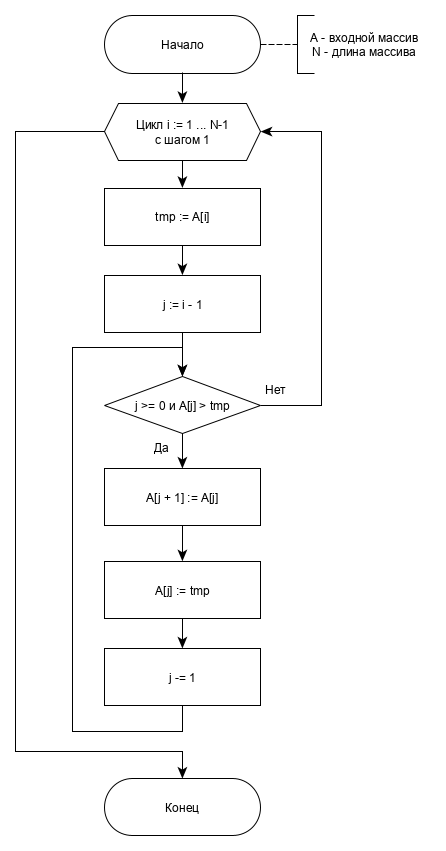
\includegraphics[scale=0.8]{insert.png}
		\caption{Сортировка вставками}
		\label{pic:insert}
	\end{figure}
	\newpage
	\begin{figure}[ht!]
		\centering
		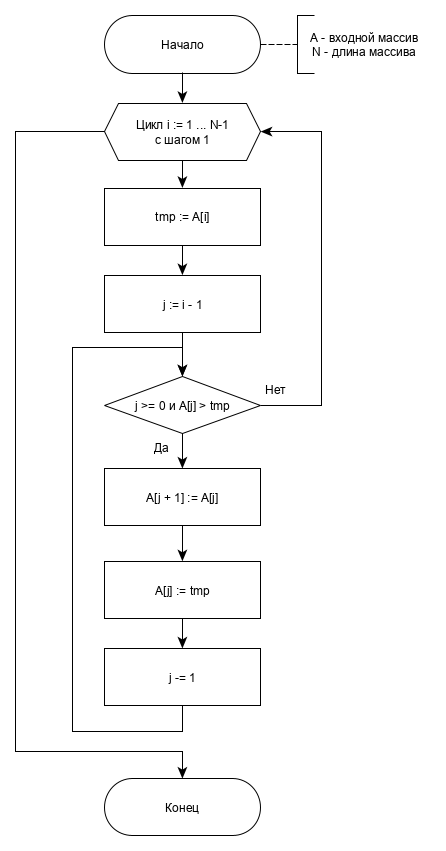
\includegraphics[scale=0.8]{insert.png}
		\caption{Сортировка слиянием}
		\label{pic:merge}
	\end{figure}
	\newpage
	\begin{figure}[ht!]
		\centering
		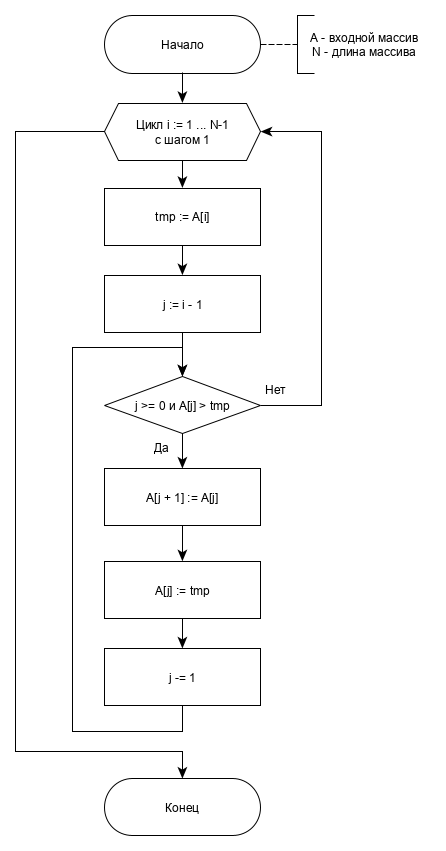
\includegraphics[scale=0.8]{insert.png}
		\caption{Быстрая сортировка}
		\label{pic:quick}
	\end{figure}

	\newpage

	\section{Оценка трудоёмкости}
	Пусть дан массив $A$ длиной $N$. Рассмотрим трудоемкость трёх алгоритмов сортировки.
	
	\subsection{Сортировка вставками}
	
	\subsection{Сортировка слиянием}
	
	\subsection{Быстрая сортировка}

	\section{Замер используемой памяти}
	Пусть дан массив $A$ длиной $N$ и для хранения целого числа требуется 4 байта памяти.\\
	В каждом из алгоритмов требуется хранить исходный массив $A$. Таким образом, под хранение массива требуется $4N$ байт памяти.\\
	
	\chapter{Технологическая часть}
	\section{Требования к программному обеспечению}
	На вход подаются размер массива и сам массив. На выход программа выдаёт три массива, которые являются результатами работы трёх различных алгоритмов сортировки. Сортировка выполняется по возрастанию.
	\section{Средства реализации}
	Для реализации программы был использован язык C++ ~\cite{CPP}. Для замера процессорного времени была использована функция rdtsc() из библиотеки stdrin.h.
	\section{Реализации алгоритмов}
	В листингах \ref{code-insert}, \ref{code-merge}, \ref{code-quick} представлены коды реализации алгоритмов сортировки массивов.
	\begin{lstlisting}[label=code-insert,caption=Сортировка вставками]
	void array_sort_insert(int * const arr, size_t n)
	{
		for (size_t i = 1; i < n; i++)
		{
			int tmp = arr[i];
			int j = i - 1;
			while (j >= 0 && arr[j] > tmp)
			{
				arr[j + 1] = arr[j];
				arr[j] = tmp;
				j--;
			}
		}
	}
	\end{lstlisting}

	\begin{lstlisting}[label=code-merge,caption=Сортировка слиянием]
	void array_merge(int * const arr, size_t first, size_t last)
	{
		size_t len = last - first + 1;
		size_t middle = (first + last) / 2;
		size_t start_1 = first;
		size_t start_2 = middle + 1;
		
		int *arr_tmp = new int[len];
		
		for (size_t i = 0; i < len; i++)
			if ((start_1 <= middle) && ((start_2 > last) ||
				(arr[start_1] < arr[start_2])))
			{
				arr_tmp[i] = arr[start_1];
				start_1++;
			}
			else
			{
				arr_tmp[i] = arr[start_2];
				start_2++;
			}
		
		for (size_t i = first; i <= last; i++)
			arr[i] = arr_tmp[i - first];
		delete [] arr_tmp;
	}
	
	void array_sort_merge(int * const arr, size_t first, size_t last)
	{
		if (first < last)
		{
			size_t middle = (first + last) / 2;
			array_sort_merge(arr, first, middle);
			array_sort_merge(arr, middle + 1, last);
			array_merge(arr, first, last);
		}
	}
	\end{lstlisting}

	\begin{lstlisting}[label=code-quick,caption=Быстрая сортировка]
	void array_sort_quick(int * const arr, size_t first, size_t last)
	{
		size_t l_hold = first;
		size_t r_hold = last;
		int pivot = arr[first];
		
		while (first < last)
		{
			while ((arr[last] >= pivot) && (first < last))
				last--;
			if (first != last)
			{
				arr[first] = arr[last];
				first++;
			}
			while ((arr[first] <= pivot) && (first < last))
				first++;
			if (first != last)
			{
				arr[last] = arr[first];
				last--;
			}
		}
		
		size_t middle = first;
		arr[middle] = pivot;
		if (l_hold < middle)
			array_sort_quick(arr, l_hold, middle - 1);
		if (r_hold > middle)
			array_sort_quick(arr, middle + 1, r_hold);
	}
	\end{lstlisting}

	\section{Тесты}
	Для проверки корректности работы были подготовлены функциональные тесты, представленные в таблице \ref{unit-tests}. Все алгоритмы должны выдавать на выходе одинаковые результаты. Сортировка выполняется по возрастанию.

	\begin{table}[ht!]
		\caption{Функциональные тесты}
		\label{unit-tests}
		\begin{center}
			\begin{tabular}{|c|c|}
			\hline
			\bf{Маccив} & \bf{Ожидание}\\\hline
			
			$\begin{bmatrix}1\end{bmatrix}$ &
			$\begin{bmatrix}1\end{bmatrix}$\\\hline
			
			$\begin{bmatrix}0 & 1 & 2 & 3 & 4 & 5 & 6 & 7 & 8 & 9\end{bmatrix}$ &
			$\begin{bmatrix}0 & 1 & 2 & 3 & 4 & 5 & 6 & 7 & 8 & 9\end{bmatrix}$\\\hline
			
			$\begin{bmatrix}9 & 8 & 7 & 6 & 5 & 4 & 3 & 2 & 1 & 0\end{bmatrix}$ &
			$\begin{bmatrix}0 & 1 & 2 & 3 & 4 & 5 & 6 & 7 & 8 & 9\end{bmatrix}$\\\hline
			
			$\begin{bmatrix}1 & 1 & 1 & 1 & 1 & 1 & 1 & 1 & 1 & 1\end{bmatrix}$ &
			$\begin{bmatrix}1 & 1 & 1 & 1 & 1 & 1 & 1 & 1 & 1 & 1\end{bmatrix}$\\\hline
			
			$\begin{bmatrix}5 & 4 & 0 & 2 & -1 & 4\end{bmatrix}$ &
			$\begin{bmatrix}-1 & 0 & 2 & 4 & 4 & 5\end{bmatrix}$\\\hline
			
			$\begin{bmatrix}5 & 4 & 0 & 2 & -1 & 3\end{bmatrix}$ &
			$\begin{bmatrix}-1 & 0 & 2 & 3 & 4 & 5\end{bmatrix}$\\\hline

			\end{tabular}
		\end{center}
	\end{table}

	В результате проверки реализации всех алгоритмов сортировки прошли все поставленные функциональные тесты.

	\chapter{Экспериментальная часть}
	\section{Примеры работы}
	На рисунке \ref{pic:example} представлен пример работы программы, демонстрирующий корректную работу алгоритмов.
	\begin{figure}[ht!]
		\centering
		\caption{Пример работы программы}
		\label{pic:example}
	\end{figure}
	
	\section{Сравнение времени работы алгоритмов}
	Для сравнения времени работы алгоритмов сортировки массивов были использованы массивы длиной от 100 до 1000 с шагом 50. Эксперимент для более точного результата повторялся 1000 раз. Итоговый результат рассчитывался как средний из полученных результатов. Результаты измерений показаны в таблице \ref{table-time} и на рисунке \ref{graph-time}.\\
	\begin{table}[ht!]
		\caption{Время работы алгоритмов сортировки массивов в тактах процессора}
		\label{table-time}
		\begin{center}
			\pgfplotstabletypeset[
			col sep=semicolon,
			string type,
			columns/Size/.style={column name=Размер массива, column type={|c}},
			columns/Insert/.style={column name=Сортировка вставками, column type={|c}},
			columns/Merge/.style={column name=Сортировка слиянием, column type={|c}},
			columns/Quick/.style={column name=Быстрая сортировка, column type={|c|}},
			every head row/.style={before row=\hline,after row=\hline},
			every last row/.style={after row=\hline},
			]{SortTime.csv}
		\end{center}
	\end{table}
	
	\begin{figure}[ht!]
		\begin{tikzpicture}
		\begin{axis}
			[%title = График времени работы алгоритмов сортировки массивов,
			table/col sep = semicolon,
			xlabel={Размер массивов},
			ylabel={Время в тиках},
			ymin = 0,
			legend pos=outer north east,
			ymajorgrids=true,
			grid style=dashed]
			\addplot[color=red, mark=*] table[x={Size}, y={Insert}] {SortTime.csv};
			\addplot[color=blue, mark=*] table[x={Size}, y={Merge}] {SortTime.csv};
			\addplot[color=green, mark=*] table[x={Size}, y={Quick}] {SortTime.csv};
			\legend{Сортировка вставками, Сортировка слиянием, Быстрая сортировка}
		\end{axis}
		\end{tikzpicture}
		\caption{График времени работы алгоритмов сортировки массивов}
		\label{graph-time}
	\end{figure}

	\newpage

	\chapter*{Заключение}
	\addcontentsline{toc}{chapter}{Заключение}
	
	...
	
	\newpage
	
	\begin{thebibliography}{}
	\bibitem{AlgAnalysis} Кормен, Т. Алгоритмы: построение и анализ / Т. Кормен, Ч. Лейзерсон, Р.М. Ривест: – МЦНТО, 1999.
	\bibitem{CPP} https://cppreference.com/ [Электронный ресурс]
	\end{thebibliography}
	\addcontentsline{toc}{chapter}{Литература}

\end{document}
